\documentclass[compress,red,mathsans,10pt]{beamer}
\usepackage{beamerthemesplit}
\usepackage{amssymb}
\usepackage{multirow}
%\usetheme{Antibes}
\usepackage{pgf,pgfarrows,pgfnodes}

\setbeamercolor{uppercol}{fg=white,bg=purple}%
\setbeamercolor{lowercol}{fg=black,bg=pink}%


\usecolortheme{lily}
\begin{document}
\title{Aplicacions Estad\'{\i}stiques}
\subtitle{Enginyeria Edificaci\'o 2009/10.}  
\author{Antonio E. Teruel}
\date{}

\frame{\titlepage} 
 
\frame{\frametitle{Exercici 1} 
En una enquesta sobre inmigraci\'o s'han obtingut les seg\"uents dades sobre la nacionalitat de 1000 persones:
\begin{center}
\begin{tabular}{c|c}
Nacionalitat & Quantitat \\ \hline
Col\'ombia & 350 \\
Equador & 250 \\
Per\'u & 120 \\
Argentina & 100 \\
Romania & 80 \\
Marroc & 70 \\
Senegal & 30
\end{tabular}
\end{center}
\begin{enumerate}[a)]
\item <1-> Representau les dades mitjan\c{c}ant una taula de freq\"u\`encies. \'es possible calcular freq\"u\`encies acumulades?
\item[] <2-> \textbf{Resp.} La taula ja \'es una taula de freq\"u\`encies. S\'{\i} \'es possible perqu\`e la variable \'es quantitativa.
\vspace{4cm}
\end{enumerate}
}

\frame{\frametitle{Exercici 1 (cont)}
\begin{enumerate}[(b)]
\item <1-> Utilitzau un diagrama de barres per a representar les freq\"u\`encies absolutes.
\item[] <2-> \textbf{Resp.} 

\begin{center}
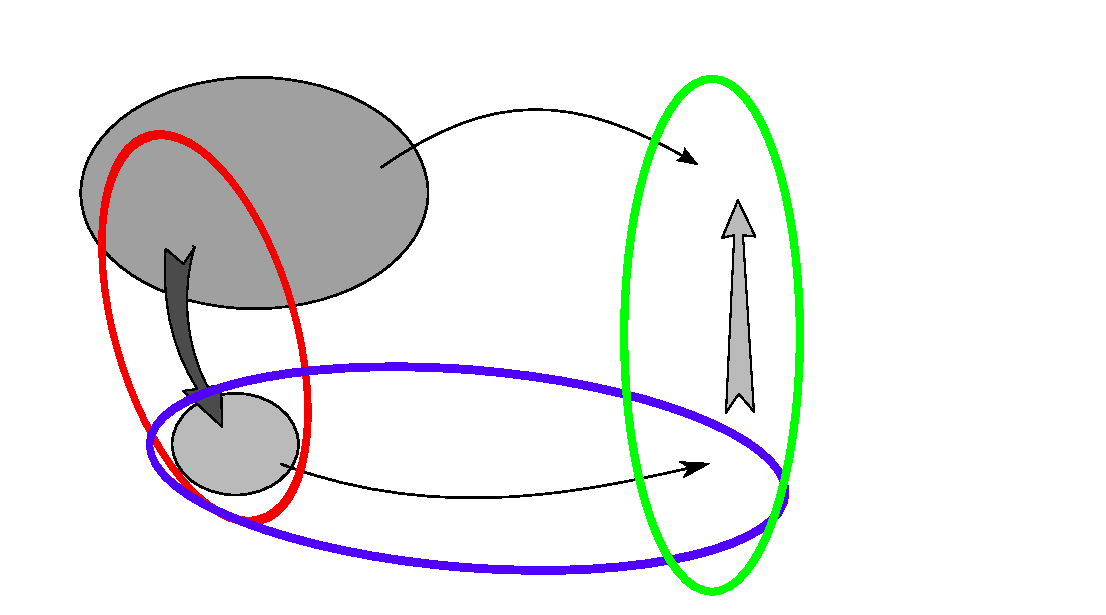
\includegraphics[width=6cm]{Dbes0108.eps}
\end{center}
\end{enumerate}
}

\frame{\frametitle{Exercici 1 (cont)}
\begin{enumerate}[(c)]
\item  <1->Representau els percentatges amb un diagrama de tarta.
\item[] <2-> \textbf{Resp.} 

\begin{center}
\includegraphics[width=6cm]{Dbes0109.eps}
\end{center}

\end{enumerate}
}

\frame{\frametitle{Exercici 2} 
En una enquesta entre els estudiants de la UIB s'han obtingut les seg\"uents dades sobre la seva edat:

\begin{center}
\begin{tabular}{|c|c|c|c|c|}
Edat & Quantitat& & Edat &Quantitat \\ \cline{1-2}\cline{4-5}
18 & 120 && 26 &  10 \\ \cline{1-2}\cline{4-5}
19 & 150 &&27 & 7 \\ \cline{1-2}\cline{4-5}
20 & 90 &&28 &  8 \\ \cline{1-2}\cline{4-5}
21 & 70 && 29 & 2\\ \cline{1-2}\cline{4-5}
22 & 65 && 30 & 1\\ \cline{1-2}\cline{4-5}
23 & 50 && 34 & 1\\ \cline{1-2}\cline{4-5}
24 & 30 && 35 & 1\\ \cline{1-2}\cline{4-5}
25 & 20 && 40 & 1\\ \cline{1-2}\cline{4-5}
\end{tabular}
\end{center}

\begin{enumerate}
\item[(a)] <1-> Representau les dades mitjan\c{c}ant una taula de freq\"u\`encies. 
\item[] <2-> \textbf{Resp.} Les dades ja est\`an en forma de taula de freq\"u\`encies. 
\end{enumerate}
}

\frame{\frametitle{Exercici 2 (cont.)} 
\begin{enumerate}
\item[(b)]<1->  Repetiu l'apartat anterior per\'o amb les dades agrupades en els seg\"uents intervals: ``Menors de $21$'', 
$[21, 23)$, $[23, 25)$, $[25, 27)$, ``Majors de $27$''.
\item[]<2-> \textbf{Resp.}

\begin{columns}
\begin{column}{0.4\textwidth}
\begin{center}
\begin{tabular}{|c|c|c|c|} \hline
Intervals&	$m_i$&	$n_i$&	$f_i$\\ \hline
Menors 21&$19$&	$360$&	$0.58$\\ \hline
$[21,23]$  &$22$&	$135$&	$0.22$\\ \hline
$[23,25]$  &$24$&	$80$&	$0.13$\\ \hline
$[25,27]$  &$26$&	$30$&	$0.05$\\ \hline
Majors 27&$35$&	$21$&	$0.03$\\ \hline
\end{tabular}
\end{center}
\end{column}
\begin{column}{0.6\textwidth}
\begin{center}
\temporal<4-5>{}{\includegraphics[width=4.5cm]{Dbes0110.eps}}
{\includegraphics[width=4.5cm]{Dbes0111.eps}}
\end{center}
\end{column}
\end{columns}

\item[(c)] <3-> Representau amb un histograma les freq\"u\`encies relatives de la taula de l'apartat anterior.
\item[(d)] <5->Obteniu el polinomi de freq\"u\`encies a partir de l'histograma anterior.
\item[]<6->
\end{enumerate}
}

\end{document}